%for reference to this section
\section{Einleitung}
\label{section:Introduction}

In den letzten Jahren hat sich die Art wie Unternehmen ihre Software hosten stark verändert. Von einfachen Virtuellen Servern bis hin zu Serverless-Applikationen, letzteres ist vor allem in den letzten Jahren stark angestiegen, da der Bedarf an schnell skalierebaren Lösungen immer wichtiger wird. Serverless-Applikationen setzen sich das Ziel große Applikationen und Programme in kleine Services aufzuteilen, die nur noch mittels Schnittstellen kommunizieren. Diese Services werden dann von dem ausgewählten Provider verwaltet, dieser bietet dann die jeweiligen Schnittstellen an, um die benötigten Features zu implementieren. Die Wartung der darunterliegenden Server wird vom jeweiligen Provider übernommen. Softwareentwicklerinnen und Softwareentwickler müssen dann nur noch ihren Programm-Code hochladen und die Services des Providers richtig konfigurieren. Dieser Programm-Code ist dann eine sogenannte Serverless Funktion, die bei beliebigen Events ausgeführt werden kann. \autocite[]{Wang}

Zurzeit gibt es jedoch noch einige Probleme mit Serverless. Das Isolieren von verschiedenen Services, beziehungsweise Funktionen gestaltet sich als schwer, da sich mehrere Container verschiedener Accounts auf den gleichen darunterliegenden Server befinden. Die Performance ist bei Serverless Funktionen sehr unberechenbar wegen der Coldstartzeiten. Diese Coldstartzeiten beschreiben die Zeit, wie lange ein Container braucht, um dessen Funktion ausführen zu können, diese variiert von Provider zu Provider und auch von Programmiersprache zu Programmiersprache \autocite[]{Wang}.
Diese Probleme könnte WebAssembly lösen, WebAssembly ist eine neue Technologie die es erlaubt Low-Level Bytecode im Browser auszuführen \autocite[]{Haas2017}. Die Ziele des WebAssembly Standard sind Sicherheit, Perfomance, Portabilität \autocite[]{Haas2017}. In der Spezifikation wird nicht explizit definiert, das WebAssembly im Browser laufen muss, und das ermöglicht es WebAssembly-Code auch auf einen Server auszuführen (zum Beispiel wasmtime \footnote{\url{https://github.com/bytecodealliance/wasmtime}}). Sogar der Co-Founder von Docker Solomon Hykes hat sich in einem Tweet geäußert, das WebAssembly die Zukunft von Server Applikationen ist. \footnote{\url{https://twitter.com/solomonstre/status/1111004913222324225?lang=de}})

Webassembly führt Low-Level Bytecode in einer eigenen Sandbox aus, die unabhängig von der darunterliegenden Host-Umgebung ist. Das führt zu einer leichteren Isolation des auszuführenden Moduls. Jedes Modul hat seinen eigenen Arbeitsspeicher, der auch unabhängig von der Host-Umgebung ist. Ein WebAssembly Modul kann somit nicht seine Umgebung, in der es ausgeführt wurde, beeinflussen. \autocite[]{Haas2017}

Die Module könnten dann als Serverless-Funktionen verwendet werden, dass hat mehrere Vorteile. Coldstartzeiten könnten verringert werden, da WebAssembly Module schneller starten können und einen kleineren Fußabdruck haben als Container oder Virtuelle Maschinen. WebAssembly hätte auch den Vorteil, das sich Programmiererinnen und Programmierer nicht nach dem Provider richten müssen, welche Programmiersprachen diese anbieten \autocite[]{Zakai2011} \autocite[]{Vilk2014} \autocite[]{LetzGRAME2017}, die jeweilige Programmiersprache müsste nur einen WebAssembly Compiler anbieten. Zurzeit gibt es erst einen Provider, der solche Serverless-Funktionen kommerziell anbietet (Cloudflare \footnote{\url{https://workers.cloudflare.com/}}).


\section{Serverless}
\label{section:Serverless}

Serverless hat vor allem in den Letzen Jahren einiges an Popularität dazugewonnen, jeder große Cloudprovider bietet mittlerweile verschiedene Serverless-Produkte an. Bei Entwicklerinnen und Entwickler wird diese Technologie auch immer beliebter.

\subsection{Serverless erklärt}

Serverless ist eine neue Cloud Computing Technologie. Bei Serverless ist das Ziel, große Applikationen in unabhängige kleine Services aufzuteilen, in dieser Seminararbeit wird vor allem der Fokus auf sogenannte Function-as-a-Service Produkte wie AWS Lambda oder Google Cloud Functions gesetzt. Bei Function-as-a-Service müssen Entwicklerinnen und Entwickler nur noch eine Funktion schreiben die einen Input und einen Output hat. Diese Funktion wird dann von den Cloud Provider ausgeführt, und der Preis wird dann pro Request berechnet. Diese Funktionen können in beliebigen Sprachen ausgeführt werden (siehe Abbildung 2). Die Serverless Funktionen werden meistens in Dockercontainer \autocite{Merkel} oder in Virtuellen Maschinen ausgeführt, somit kann eine Isolation zwischen verschiedenen Funktionen erreicht werden \autocite[]{Zakai2011}. Diese Isolation ermöglicht es den Cloud Provider mehrere Funktionen auf einer Host Umgebung zu starten, ohne das diese sich gegenseitig beeinflussen, wenn eine Funktion eine gewisse Zeit nicht mehr aufgerufen wurde, wird dessen Container terminiert und muss bei einem neuen Request neu gestartet werden, das nennt man dann den Coldstart \autocite[]{Lloyd}). \autocite[]{Muthusamy2017}


\subsection{Vorteile von Serverless}

\begin{flushleft}

\textbf{Skalierbarkeit:} Eine Applikation aufzubauen, die eine hohe Skalierbarkeit und Verfügbarkeit hat, ist eine sehr teure und aufwändige Aufgabe, wenn man diese konventionell löst \autocite[]{Ma} \autocite[]{Bryhni}. Bei Serverless werden alle Services automatisch von dem jeweiligen Cloud Provider skaliert, und der Preis wird dynamisch anhand der Requestzahlen oder verbrauchten Ressourcen von den verschiedenen Services errechnet. \autocite[]{Muthusamy2017} \break


\textbf{Reduzierte Kosten:} Die Kosten von Serverless Applikationen werden immer dynamisch anhand der Requestzahlen beziehungsweiße an den verbrauchten Resourcen errechnet \autocite[]{VanEyk2017} \autocite[]{Malawski}. Das ist bei kleinen Projekten oder Unternehmen, die nicht das ganze Jahr die gleiche Auslastung haben vom Vorteil. Zusätzlich gibt es bei den meisten Cloud Providern ein Freetier, somit können ganz kleine Projekte fast kostenlos umgesetzt werden. \break



\textbf{Kürzere Entwicklungzeit:} Der größte Vorteil von Serverless ist der verringerte Aufwand. Cloud Provider verwalten die unter Serverless liegende Serverarchitektur. Entwicklerinnen und Entwickler müssen somit keine Zeit für die Wartung der vorhandenen Server Architektur aufwenden, sondern können sich auf das Weiterentwickeln des Produktes kümmern. \autocite[]{Baldini}

\end{flushleft}

\begin{figure}[t]
	\centering
	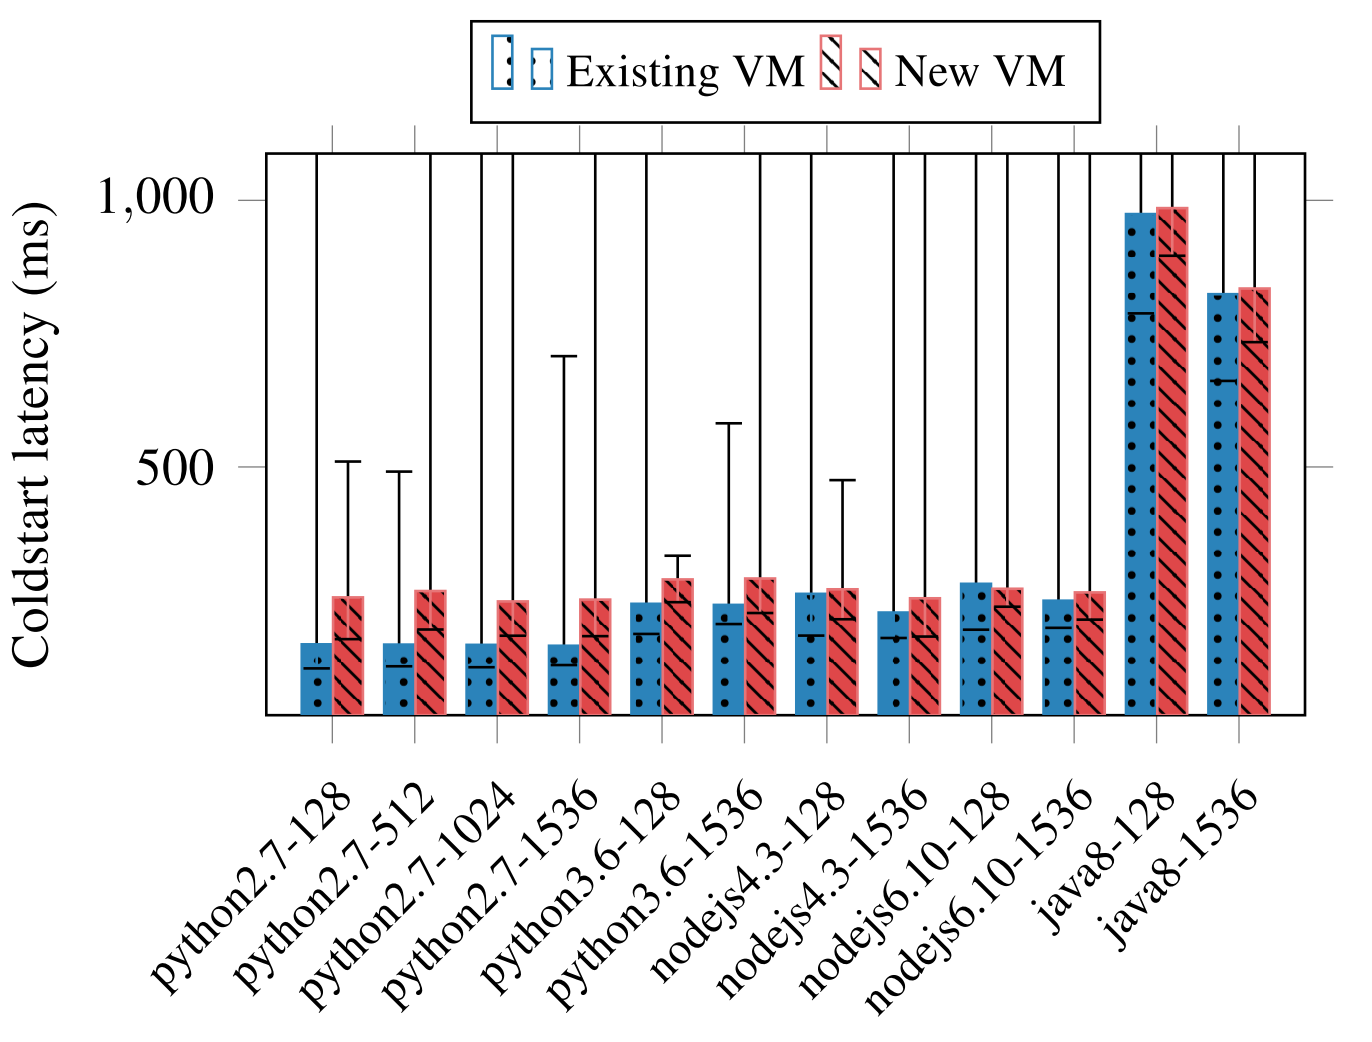
\includegraphics[width=0.5\textwidth]{images/Coldstarts.png}
	\caption{
		Coldstartzeiten von AWS Lambda \autocite[]{Wang}
	}
	%for reference to this figure
	\label{figure:Coldstarts}
\end{figure}

\subsection{Probleme von Serverless}

\begin{flushleft}
\textbf{Coldstartzeiten:} Coldstartzeiten sind ein großes Performance Problem bei Functions-as-a-Service. \autocite[]{Lloyd} Jedes Mal wenn eine Funktion nicht mehr gebraucht wird, wird der Container oder die Virtuelle Maschine vom Cloud Provider wieder gelöscht und erst beim nächsten Request wieder gestartet. Das führt zu einer längeren Request Zeit, diese zusätzliche Zeit hängt von der Programmiersprache und deren Runtime ab. Um diesen Performance Problem entgegen zu wirken cachen die Cloud Provider die Container oder Virtuellen Maschinen für eine gewisse Zeit. \autocite[]{Hall2019} Abbildung 1 zeigt die verschiedenen Coldstartzeiten von AWS Lambda. \break

Das Paper \autocite[]{Wang} beschäftigt sich mit Coldstartzeiten von AWS Lambda. Es wurde herausgefunden, dass es einen Unterschied macht, ob die Virtuelle Maschine bereits einmal gestartet wurde oder komplett neu ist, dieser Unterschied ist im Durchschnitt 39 ms. Python hat die niedrigsten Coldstarts (167 – 171 ms) von den getesteten Programmiersprachen. Java hat die höchste Coldstart Latenz (824 – 974ms). Der große Unterschied zwischen den Sprachen könnte damit erklärt werden, dass AWS CPU Leistung proportional zum Arbeitsspeicher allokiert wird, das heißt, je mehr Arbeitsspeicher eine Funktion benötigt, desto mehr Zugriff auf CPU Leistung hat diese, und kann somit Programmierumgebungen schneller starten. Zusätzlich wurde herausgefunden, dass wenn man mehrere Funktionen auf einer Virtuellen Maschine startet, die Coldstart-Latenz auch nach oben geht. \break


\textbf{Abhängigkeit von Cloud Provider:} Wenn man eine Server Architektur für eine Web-Applikation selbst aufbaut braucht man lediglich einen Virtuellen Server von einem Provider und falls man sich später für einen anderen Anbieter entscheidet, ist dieser Umzug nicht allzu schwer. Jedoch mit Serverless, vor allem wenn man viele verschiedene Services des Providers verwendet, kann sich das als äußert schwierig herausstellen, es kann sein das die gesamte Codebase für diesen neuen Cloud Provider umgebaut werden muss. \autocite[]{VanEyk2017} \break


\textbf{Schwierig zu testen:} Testen gestaltet sich als schwierig, vor allem lokale Tests sind fast unmöglich, da die gesamte Infrastruktur lokal nur sehr schwierig abgebildet werden kann. Manche Tests lassen sich erst nach den Deployment durchführen, was dazu führen kann, das fehlerhafte Builds released werden. \autocite[]{Manner2019} \break 

\end{flushleft}

\begin{figure*}[ht]
	\centering
	\begin{tabular}{r|rrrrrrr}
		                  & $JavaScript$ & $Python$ & $Ruby$ & $Java$ & $Go$ & $C\#$ & $F\#$ \\ \hline
		$AWS\ Lambda$      & $Ja$         & $Ja$     & $Ja$   & $Ja$   & $Ja$ & $Ja$ & $Nein$ \\
		$Azure\ Functions$ & $Ja$         & $Ja$     & $Nein$ & $Ja$   &$Nein$& $Ja$ & $Ja$ \\
		$Google\ Cloud\ Functions$ & $Ja$ & $Ja$ & $Nein$ & $Nein$ & $Ja$ & $Nein$ & $Nein$
	\end{tabular}
	\caption{
		Tabelle der verschiedenen Programmiersprachen der Cloud Provider
	}
	\label{table:ProgrammingLang}
\end{figure*}

\section{WebAssembly}
\label{section:WebAssembly}

WebAssembly ist ein Binary Code Format, das speziell für Browser entwickelt wurde, es erlaubt Low-level Code in Web auszuführen. Laut Spezifikation funktioniert WebAssembly aber auch außerhalb von Browsern \footnote{\url{https://webassembly.github.io/spec/core/bikeshed/}}. WebAssembly ist vor allem der einzige Standard in diesen Bereich, der von allen größeren Browserherstellern unterstützt wird.

\subsection{WebAssembly Vorgänger}

Es gab schon einige Vorgänger von WebAssembly, die versuchten Low-level Code im Browser ausführbar zu machen, die meisten würden jedoch wegen verschiedener Probleme nie in allen Browsern implementiert. \autocite[]{Haas2017}

\begin{flushleft}

\textbf{Native Client} war das erste System, das mittels Sandboxing Maschinen-Code \autocite[]{Yee2010} im Web ausführen konnte. Native Client konnte in Google Chrome jedoch nicht so implementiert werden, dass es sich im gleichen Prozess befindet, und deswegen kann man nicht auf diverse Web- und JavaScript-APIs zugreifen. Dass Native Client nicht direkt im gleichen Prozess laufen konnte liegt vor allem an verschiedenen Einschränkungen im Google Chrome Browser. \autocite[]{Haas2017} Zusätzlich war Native Client oder NaCl nicht portierbar, da es auf einem sehr architekturspezifischen Maschinencode basierte. Später wurde dann der Portable Native Client \autocite[]{Donovan2010} entwickelt, der auf LLVM bytecode basiert und somit architekturunabhängig war. Es würden jedoch immer noch sehr viele Plattformspezifische Details offengelegt. NaCl und PNaCl wurden lediglich in Google Chrome implementiert.

\hfill \break

\textbf{Emscripten} kompiliert C/C++ Applikationen zu einen spezialisierten Subset von JavaScript (asm.js \footnote{\url{http://asmjs.org/}}). Asm.js ist ein Subset von JavaScript, das vor allem die JavaScript Spezifikation ausnützt, um gewisse Performancesteigerungen zu erzielen. Mittlerweile kompiliert Emscripten zu WebAssembly. \autocite[]{Zakai2011}

\hfill \break

\textbf{Java und Flash} stellten Runtime-Plugins für Browser bereit, diese aber jedoch unterstützen keinen Low-Level Code, und heutzutage werden diese beiden Plugins aus Sicherheit und Performance Gründen nicht mehr verwendet. \autocite[]{Haas2017}

\end{flushleft}


\subsection{WebAssembly erklärt}

\begin{figure*}[t]
	\centering
	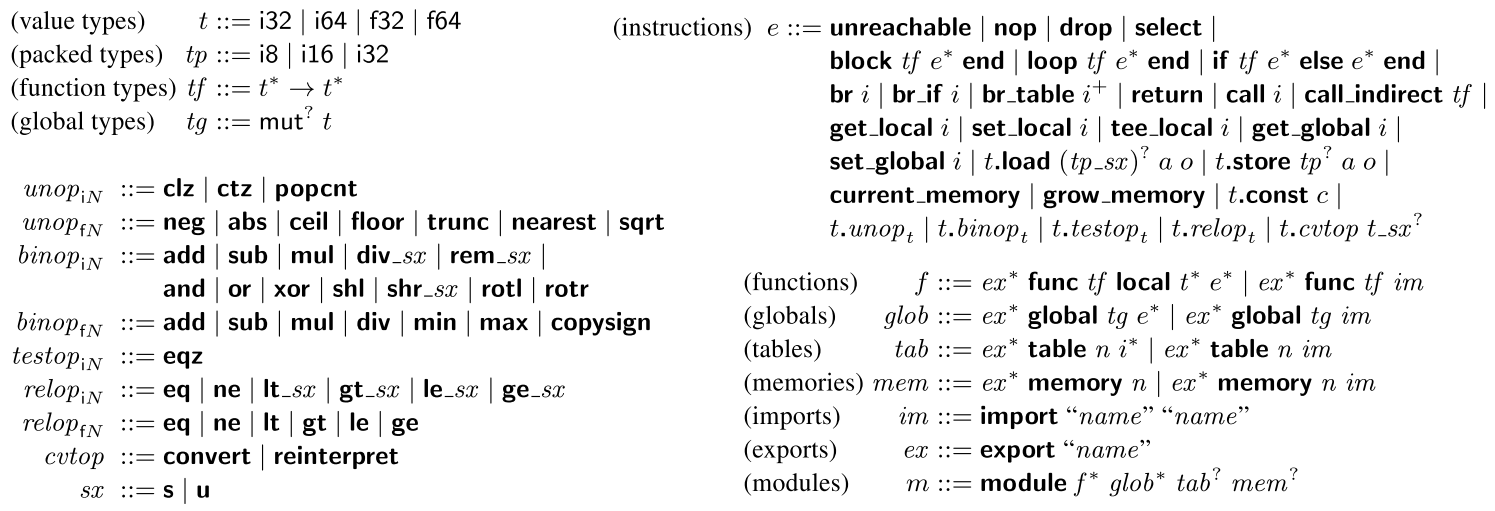
\includegraphics[width=1\textwidth]{images/WebAssemblySyntax.png}
	\caption{
		WebAssembly Syntax \autocite[]{Haas2017}
	}
	%for reference to this figure
	\label{figure:WASyntax}
\end{figure*}

WebAssembly Byte-Code besteht aus verschiedenen Komponenten (siehe Abbildung 3).


\begin{flushleft}
\textbf{Module}: Umfassen das gesamte Binary, also ein Modul beinhaltet mehrere Deklarationen von Funktionen, Globals, Tables, und Memories \autocite[]{Haas2017}. Diese Deklarationen können dann unter verschiedenen Namen exportiert oder importiert werden. Das Module kann dann vom jeweiligen Embedder, zum Beispiel JavaScript importiert werden. \autocite[]{Haas2017}

\hfill \break

\textbf{Funktionen}: Eine Funktion nimmt eine beliebige Anzahl an Parametern und gibt welche zurück. Funktionen können nicht inereinander verschachtelt werden. Funktionen können von anderen Funktionen und auch rekursiv aufgerufen werden. \autocite[]{Haas2017}

\hfill \break

\textbf{Instruktionen}: Instruktionen sind verschiedene Operationen, die bestimmte Werte und Speicher bearbeiten können, diese werden innerhalb der Funktionen ausgeführt. \autocite[]{Haas2017}

\hfill \break

\textbf{Traps}: Falls eine Instruktion einen Fehler verursacht, kann eine Trap ausgelöst werden, die zum sofortigen Abbrechen des Programmes führt. Diese Traps müssen vom jeweiligen Embedder behandelt werden, in JavaScript wird eine Exception mit dem JavaScript und WebAssembly Stacktrace geworfen. \autocite[]{Haas2017}

\hfill \break

\textbf{Typen}: WebAssembly Bytecode hat nur 4 verschiedene Basis Variablen Typen, Integer und Floating Point Number, diese in einer 32 und 64bit Version. WebAssembly hat keine Unterscheidung zwischen signed und unsigned Integer, falls es jedoch für die Berechnung wichtig ist kann \_u oder \_s als Suffix hinzugefügt werden. \autocite[]{Haas2017}

\hfill \break

\textbf{Lokale Variablen}: Funktionen können lokale Variablen deklarieren, diese könen mittels der \textbf{get\_local} und \textbf{set\_local} Instruktion gesetzt oder gelesen werden. \autocite[]{Haas2017}

\hfill \break

\textbf{Globale Variablen}: Es können auch Variablen global in einem Modul deklariert werden, diese können dann in mehreren Funktionen verwendet werden. \autocite[]{Haas2017}

\hfill \break

\textbf{Memory Managment:} In WebAssembly werden alle Variablen und Werte in einem Array von Bytes gespeichert, diesen Array bezeichnet man als Memory oder linear Memory. Ein Modul hat jeweils einen Memory Array, dieser wird mit einer bestimmten Größe initialisiert, kann aber im Laufe des Programmes dynamisch erweitert werden. Falls es zu einem Out-of-Memory Fehler kommt gibt die Instruction \textbf{grow\_memory}, die verwendet wird, um den Speicher dynamisch zu erweitern, den Wert -1 zurück. Der Speicher wird immer um 64KiB erweitert. 
Um auf den Speicher mittels \textbf{load} zuzugreifen, wird die eine dynamische i32 Adresse benötigt. Speicher Adressen sind unsigned 32 bit integer die bei 0 starten. Es können immer 8, 16, 32 und 64bit aus dem Speicher geladen werden.
Der Lineare Speicher ist komplett vom Code und Execution Stack getrennt, das heißt, dass ein fehlerhaftes WebAssembly Programm nicht sein Execution Environment verändern kann, ein fehlerhaftes Programm kann nur dessen eigenen Speicher manipulieren. Dadurch, dass der Speicher so isoliert ist, können auch nicht vertrauenswürdige WebAssembly Module ausgeführt werden, und WebAssembly kann auch in anderen Sprachen implementiert werden, ohne dessen Speichermanagement zu verändern. \autocite[]{Haas2017} \autocite[]{Ansel2011} \break

\textbf{Syntax} Die meisten Assembler Sprachen springen meistens von Instruktion zu Instruktion, WebAssembly hingegen verhält sich wie eine Programmiersprache. WebAssembly implementiert einen sogenannten Structured Control Flow. WebAssembly kann somit besser die Validität des Programmes feststellen, zusätzlich kann jedes Modul in einen Durchgang validiert und kompiliert werden.
Manche Sprachen Konstrukte müssen mit \textbf{end} geschlossen werden, zum Beispiel \textbf{block}, \textbf{if} und \textbf{loop}. \autocite[]{Haas2017}

\end{flushleft}

\subsection{Ziele von WebAssembly}

WebAssembly versucht gleichzeitig das Beste seiner Vorgänger zu verwenden, aber vor allem ist das Ziel deren Probleme zu lösen.

\begin{flushleft}


\textbf{Sicherheit}: Sicherheit ist ein großer Faktor im Web, da sehr viel Programm-Code aus nicht vertrauenswürdigen Quellen stammt. Eine Low-Level Sprache im Web muss vor allem unabhängig von der Umgebung, in der sie ausgeführt wurde, laufen, um Memory Leaks und dergleichen zu verhindern. \autocite[]{Haas2017}

\hfill \break

\textbf{Performance}: Low-Level Code kann direkt ausgeführt werden, das beschleunigt das Ausführen des Programmes enorm. Programmiersprachen wie JavaScript müssen jedoch zur Laufzeit noch in einen Low-Level Code kompiliert werden, und das kostet Zeit. \autocite[]{Haas2017}

\hfill \break

\textbf{Portable}: Im Web werden verschiedenste Geräte verwendet, von billigen Smartphones bis leistungsstarken Rechnern. Ein Low-Level Bytecode sollte auf jeder Architektur laufen, er sollte auch in jeden großen Browser implementiert werden. Um das zu erreichen, muss dieser unabhängig von Betriebssystem, Browser und Hardware sein. \autocite[]{Haas2017}

\hfill \break

\textbf{Kompakt}: Da dieser Low-Level Code über das Netzwerk ausgeliefert wird, sollte er so kompakt wie möglich sein, um Bandbreite zu sparen. \autocite[]{Haas2017}

\end{flushleft}

\begin{figure}[t]
	\centering
	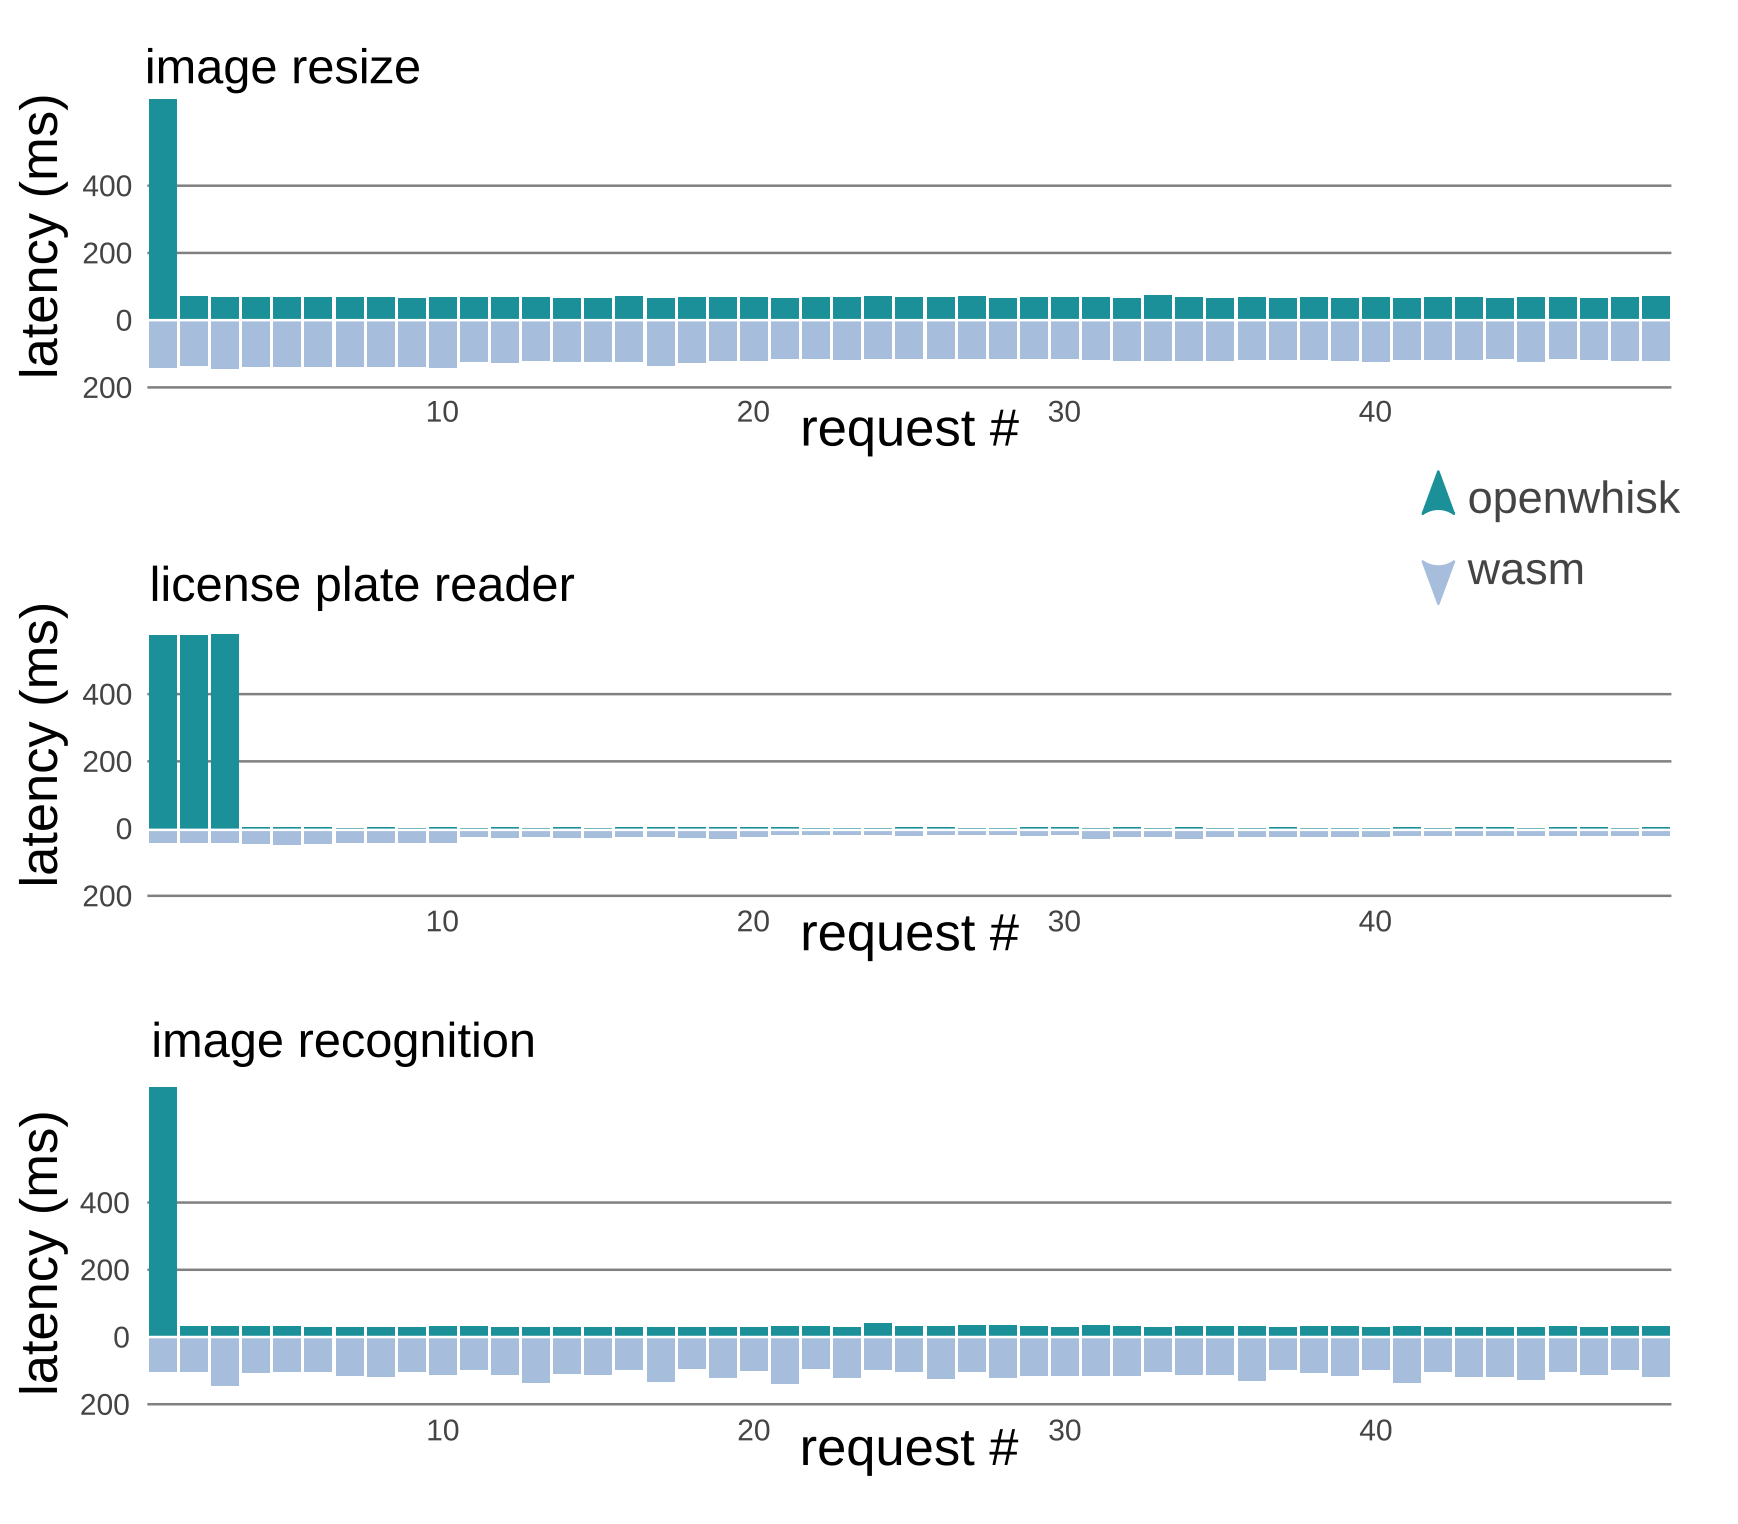
\includegraphics[width=0.5\textwidth]{images/RequestTimesSlow.png}
	\caption{
		Startup Latenzen OpenWhisk vs. WebAssembly \autocite[]{Hall2019}
	}
	%for reference to this figure
	\label{figure:StartupLatFirst}
\end{figure}

\begin{figure}[t]
	\centering
	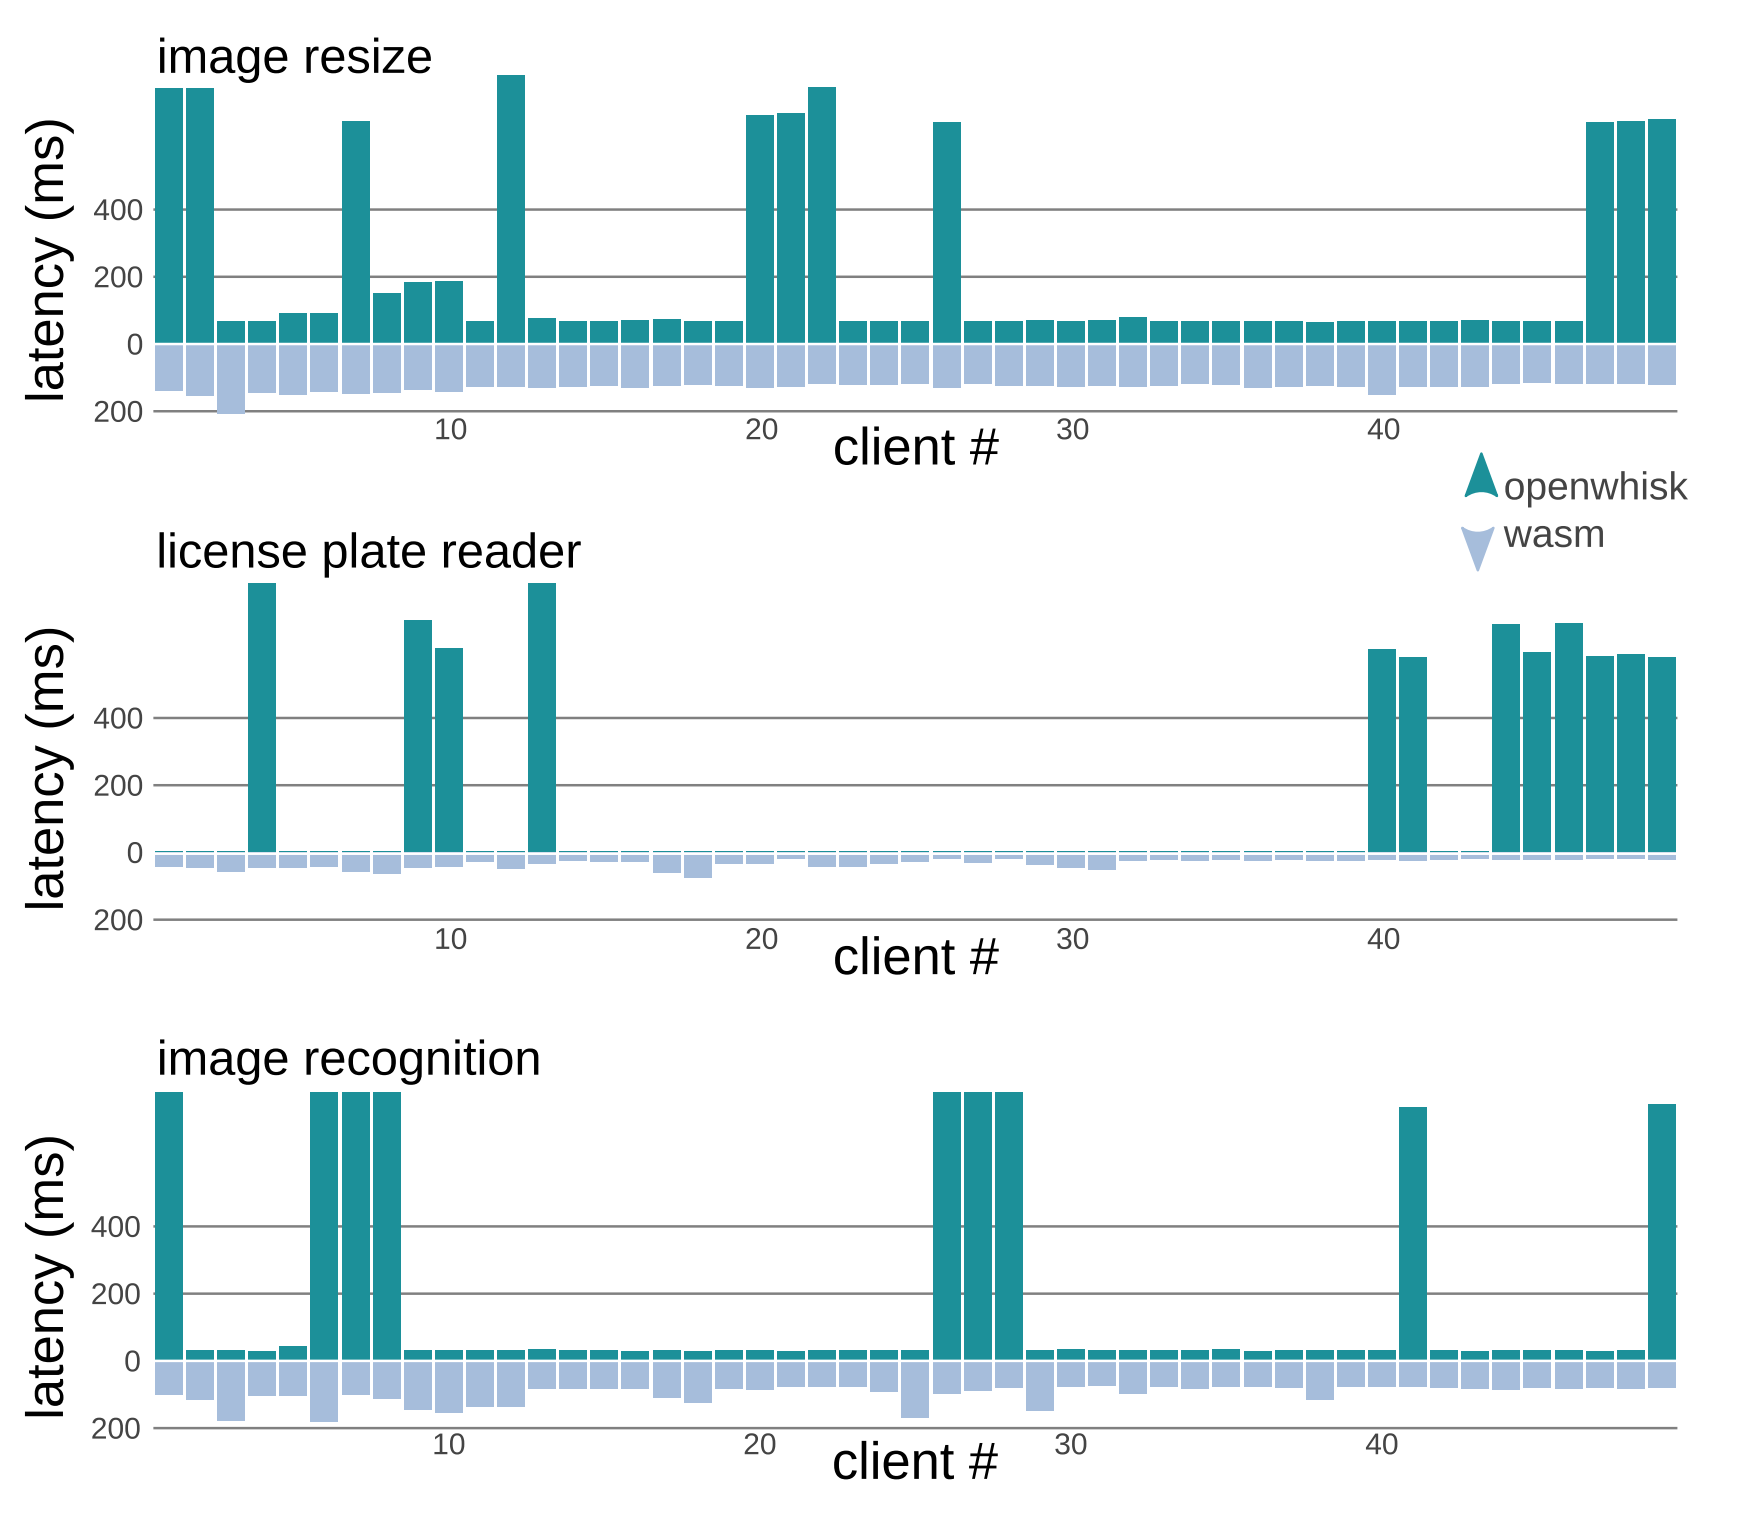
\includegraphics[width=0.5\textwidth]{images/RequestTimesReal.png}
	\caption{
		Startup Latenzen OpenWhisk vs. WebAssembly \autocite[]{Hall2019}
	}
	%for reference to this figure
	\label{figure:StartupLatSecond}
\end{figure}

\section{Serverless mit WebAssembly}
\label{section:Serverless mit WebAssembly}

Serverless hat noch einige Probleme \autocite[]{Baldini}, diese wurden im Punkt 2.3 Probleme von Serverless in dieser Arbeit genau erläutert. WebAssembly hat einige Eigenschaften, die zur Lösung dieser Probleme beitragen könnten, und mehrere Firmen und Arbeiten beschäftigen sich bereits mit dieser Thematik. Anbieter wie Cloudflare \footnote{\url{https://workers.cloudflare.com/}} bieten mittlerweile Produkte an, die WebAssembly nützen, um genau diese Probleme zu lösen. Anbieter wie Cloudflare haben vor allen den Vorteil von einem großen Netzwerk, das aber pro Rechenzentrum nicht so leistungsstark ist wie zum Beispiel ein Rechenzentrum von Amazon Web Services. Diese Anbieter konnten davor nicht Serverless Produkte anbieten, da diese zu rechenintensiv waren, doch mit WebAssembly kann der Overhead drastisch reduziert werden. \autocite[]{Hall2019}

\subsection{Coldstarts}

Bei den derzeitigen großen Serverless Providern liegt die Coldstartzeit zwischen 500ms und 800ms \autocite[]{Shilkov} (alle Programmiersprachen, für genauere Daten \autocite[]{Wang}). Diese könnte mittels WebAssembly reduziert werden. Das Problem, warum diese Coldstartzeiten so hoch sind, ist vor allem Docker \autocite[]{Merkel}, denn bei jedem Coldstart muss ein neuer Dockercontainer gestartet werden, das kostet Zeit, auch wenn man diesen Prozess so effizient wie möglich gestaltet. Die WebAssembly Spezifikation erwähnt nicht explizit den Browser als Embedder von WebAssembly \autocite[]{Haas2017}, es kann auch WebAssembly außerhalb des Browsers ausgeführt werden und durch das Sandboxing können verschiedene WebAssembly Module voneinander isoliert ausgeführt werden, ähnlich wie bei einem Dockercontainer. Dadurch, dass WebAssembly nur Low-Level Bytecode \autocite[]{Zakai2011} ist, können die WebAssembly Module schnell starten. Coldstarts mittels WebAssembly liegen bei (Angabe von kommerziellen Anbieter Cloudflare) 5ms.

In diesem Paper \autocite[]{Hall2019} werden herkömmliche Serverless Funktionen und WebAssembly Module verglichen. Als Serverless-Backend wurde OpenWhisk \footnote{\url{https://openwhisk.apache.org/}} verwendet. Hier fällt auf das OpenWhisk bei einem Warmstart um 1.5 - 3x schneller ist als WebAssembly (Single Client, Single Access Workload). Jedoch ist bei OpenWhisk der erste Request (Coldstart) um einiges langsamer. Diese Coldstarts passieren bei einem realistischen Workload jedoch viel öfter, in Abbildung 4 sieht man, wie die gleiche Funktion mehrfach hintereinander in der Sekunde aufgerufen wird, hier ist im Durchschnitt OpenWhisk schneller. In Abbildung 5 wurde eine realistischere Workload (Multiple Client, Multiple Access Workload) verwendet, und hier sieht man dass WebAssembly im Durchschnitt schneller ist. WebAssembly verhält sich viel berechenbarer als OpenWhisk, mit fast konstanten Requestzeiten. Dieses Paper wurde im Kontext von IoT \footnote{Internet of Things} Geräte geschrieben, um herauszufinden, ob mehr Request pro Sekunde mit WebAssembly oder mit OpenWhisk abgearbeitet werden können. 



\subsection{Programmiersprachen unabhängig}

Eines der Probleme von Serverless war, dass man oft von Cloud Providern abhängig ist, und auch deren Programmiersprachen wählen muss, diese Provider bieten nicht alle Programmiersprachen an. Dieses Problem der Programmiersprachen-Abhängigkeit kann auch mittels WebAssembly gelöst werden. Jeder Cloud Provider unterstützt WebAssembly Module, da es in den neueren Versionen von NodeJs implementiert ist, das erlaubt es WebAssembly Module in JavaScript zu importieren. Somit muss man nur den Code aus einer beliebigen Programmiersprache zu einem WebAssembly Module kompilieren und kann jede beliebige Sprache verwenden \autocite[]{Vilk2014} \autocite[]{LetzGRAME2017}.

\section{Fazit}

Serverless Funktionen beziehungsweiße ganze Serverless-Applikationen können einiges an Arbeit verringern. Es ist jedoch um einiges komplizierter zum Lernen und viel abstrakter als ein einfacher virtueller Server. Zusätzlich dazu gibt es zurzeit viele Frameworks wie Symfony, Ruby on Rails oder Laravel, die viel erleichtern, mit Serverless muss man diese Dienste entweder als Service von einem Cloud Provider hinzufügen oder selbst implementieren, das jedoch nicht immer mit Serverless Funktionen möglich ist, zum Beispiel Bilder, die für immer abgespeichert werden sollen. Serverless ist im Großen und Ganzen eine gute Ergänzung für die derzeitige Serverlandschaft, und vor allem für kleine Projekte und Projekte mit schwankender Auslastung, ist Serverless sehr gut geeignet. Das größte Problem von Serverless ist in meinen Augen zurzeit die Abhängigkeit von den jeweiligen Cloud Providern, denn wenn man sich für einen Provider entscheidet, ist es später sehr schwierig die komplette Applikation umzuziehen, da die verschiedenen Services von den verschiedenen Providern alle anders über die Schnittstellen angesprochen werden. Und somit müsste man einen großen Teil des Programm-Codes umschreiben. Ein weiteres Problem ist auch die fehlende Transparenz der verschiedenen Provider, und wie diese genau ihre Services hosten.

Durch WebAssembly gibt es jetzt einen Low-Level Bytecode, der in einem Browser in einer isolierten Sandbox ausgeführt werden kann, und die oben genannten Kriterien erfüllt \autocite[]{Haas2017}. Das wichtigste Feature ist die Plattform Unabhängigkeit, die es ermöglicht WebAssembly überall auszuführen. Zusätzlich kann jede Programmiersprache in ein WebAssembly Modul kompiliert werden, somit kann man Software-Bibliotheken, die in JavaScript schlechter, beziehungsweise nicht implementiert wurden, einfach zu einem WebAssembly Modul kompilieren und im Browser verwenden, zum Beispiel Kryptographische-Bibliotheken \autocite[]{Renner} oder Bildverarbeitungs-Bibliotheken.

Wenn man WebAssembly mit Serverless kombiniert können einige Probleme von Serverless gelöst werden \autocite[]{Baldini} und manche Cloud Provider beweisen dies auch. \cite{Hall2019} zeigen zwar das Serverless Plattformen wie OpenWhisk bei Warmstarts schneller sind als WebAssembly, jedoch haben sie eine hohe Coldstart-Latenz, und da in einer realen Anwendung öfter Coldstarts vorkommen wäre WebAssembly hier berechenbarer und im Durchschnitt schneller.